\documentclass[11pt]{article}

\usepackage[T1]{fontenc}
\usepackage{lmodern}
\usepackage{microtype}
\usepackage[a4paper,margin=28mm]{geometry}
\usepackage{amsmath,amssymb,amsthm,mathtools}
\usepackage{booktabs}
\usepackage{tabularx}
\usepackage{graphicx}
\usepackage{xcolor}
\usepackage{enumitem}
\usepackage{hyperref}

\definecolor{linkblue}{HTML}{1B4965}
\hypersetup{
  colorlinks=true,
  linkcolor=linkblue,
  citecolor=linkblue,
  urlcolor=linkblue,
  pdftitle={From finite-game operators to dense numerical linear algebra},
  pdfauthor={Davide Legacci}
}

\graphicspath{{experiments/}}
\setlength{\parindent}{0pt}
\setlength{\parskip}{0.55em}
\setlist{nosep,leftmargin=*}

\newtheorem{proposition}{Proposition}
\newtheorem{lemma}{Lemma}
\newtheorem{remark}{Remark}
\newtheorem{definition}{Definition}

\newcommand{\R}{\mathbb{R}}
\newcommand{\one}{\mathbf{1}}
\newcommand{\diag}{\operatorname{diag}}
\newcommand{\range}{\operatorname{range}}
\newcommand{\rank}{\operatorname{rank}}
\newcommand{\cO}{\mathcal{O}}
\newcommand{\ip}[2]{\left\langle #1,#2\right\rangle}

\title{From Finite-Game Operators to Dense Numerical Linear Algebra\\
\large A computational account of the maintained potential--harmonic decomposition}
\author{Davide Legacci}
\date{July 2026}

\begin{document}

\maketitle

\begin{abstract}
This note documents the computational realization of the finite-game
decomposition implemented in
\path{CandoganDecomposition/decomposition.py}.  It does not reproduce the
structural theory of potential, harmonic, and nonstrategic games developed by
Candogan et al. or its weighted formulation by Abdou et al.  Instead, it gives
the complete bridge from the abstract operators used by that theory to the
arrays and dense linear-algebra operations executed by the program.  We define
the profile and edge indexings, derive every stored matrix, identify the sole
Moore--Penrose pseudoinverse formed by the maintained implementation, and show
how normalization and the exact-flow projection are applied without building
their full matrices.  We then derive time and storage bounds in terms of the
number of players, profiles, and response edges.  Finally, a reproducible
benchmark on weighted random games measures geometry construction and cached
decomposition separately.  The data expose the expected exponential scaling
in the number of players and the practical memory cost of storing dense
incidence and gradient matrices.
\end{abstract}

\tableofcontents

\section{From abstract operators to program operations}
\label{sec:implementation}

\subsection{Scope and conventions}

The theory is taken from Candogan et al.~\cite{candogan2011} in the uniform
case and Abdou et al.~\cite{abdou2022} in the weighted case.  Only the formulas
needed to identify a theoretical object with a concrete program operation are
recalled.  In particular, no attempt is made to reprove the decomposition
theorem.

Let there be $n\geq 1$ players.  Player $i$ has the finite action set
\[
 A_i=\{0,1,\ldots,d_i-1\},\qquad d_i\geq 1,
\]
and the pure-profile set is
\[
 A=\prod_{i=1}^n A_i,\qquad M=|A|=\prod_{i=1}^n d_i.
\]
The input measures are vectors
\[
 \mu_i=(\mu_i(0),\ldots,\mu_i(d_i-1)),\qquad \mu_i(a_i)>0.
\]
Strict positivity is checked by the constructor.  If no measures are supplied,
the program sets every entry to one.  Measures are not normalized.  Define
\[
 m_i=\sum_{a_i\in A_i}\mu_i(a_i),\qquad
 p(a)=\prod_{i=1}^n\mu_i(a_i),\qquad
 \mu_{-i}(a_{-i})=\prod_{j\neq i}\mu_j(a_j).
\]
The maintained interface does not accept a separate opponent comeasure
$\gamma$; the implemented convention is $\gamma_i\equiv 1$.

A game is represented by a real tensor
\[
 u\in\R^{n\times d_1\times\cdots\times d_n},
\]
where $u_i(a)$ is stored at \texttt{payoffs[i, a1, ..., an]} after converting
the mathematical player index to Python's zero-based index.  A flat vector of
length $nM$ is also accepted and reshaped in NumPy C order.  In the formulas
below, the profile index is
\[
 \kappa(a_1,\ldots,a_n)
 =\sum_{i=1}^n a_i\prod_{j=i+1}^n d_j
 \in\{0,\ldots,M-1\}.
\]
This is NumPy C-order indexing.  The program uses \texttt{np.ndindex} to
enumerate profiles, \texttt{reshape} to interpret flat payoffs, and
\path{np.ravel_multi_index} to map profile tuples to columns.

\subsection{The oriented response graph}

Two profiles are response adjacent for player $i$ when they agree in every
coordinate except coordinate $i$.  The code stores one orientation of every
undirected response edge.  For each opponent profile $a_{-i}$ and each pair
$0\leq r<s<d_i$, it stores
\[
 e=(i,a^-,a^+),\qquad
 a^-=(r,a_{-i}),\quad a^+=(s,a_{-i}),
\]
with the entries inserted in their correct coordinate positions.  The number
of player-$i$ edges and total edges are therefore
\begin{equation}
 E_i=\frac{M}{d_i}\binom{d_i}{2}
    =\frac{M(d_i-1)}{2},\qquad
 E=\sum_{i=1}^nE_i
  =\frac{M}{2}\sum_{i=1}^n(d_i-1).
 \label{eq:edge-count}
\end{equation}
Every two profiles can be connected by changing their coordinates one at a
time, so the response graph is connected, including the trivial one-vertex
case.

Fix the program's edge ordering.  Its dense incidence matrix
$B\in\R^{E\times M}$ is
\begin{equation}
 B_{e,c}=
 \begin{cases}
 -1,&c=\kappa(a^-),\\
 +1,&c=\kappa(a^+),\\
 0,&\text{otherwise}.
 \end{cases}
 \label{eq:incidence}
\end{equation}
Thus each row contains exactly two nonzero entries, although the implementation
stores all $EM$ entries as double-precision numbers.  The arrays
\texttt{edge\_players}, \texttt{edge\_tails}, and \texttt{edge\_heads} store
the corresponding integer metadata.

\subsection{Weighted profile and flow spaces}

Define the diagonal profile-weight matrix
\[
 P=\diag\bigl(p(a):a\in A\bigr)\in\R^{M\times M}.
\]
For an edge $e=(i,a^-,a^+)$ define
\[
 s_e=\mu_{-i}(a_{-i})^{-1/2},\qquad
 q_e=p(a^-)p(a^+).
\]
Let
\[
 S=\diag(s_e:e\in E),\qquad Q=\diag(q_e:e\in E).
\]
The weighted gradient matrix is
\begin{equation}
 G=SB\in\R^{E\times M}.
 \label{eq:gradient-matrix}
\end{equation}
Consequently, for $f\in\R^M$,
\[
 (Gf)_e=s_e\bigl(f(a^+)-f(a^-)\bigr).
\]

The program stores the diagonal entries of $P$, $Q$, and $S$ as the vectors
\texttt{profile\_weights}, \texttt{flow\_weights}, and
\texttt{gradient\_scales}.  It does not allocate the three diagonal matrices.
Multiplication by a diagonal matrix is implemented as elementwise vector
multiplication.  It does allocate the dense matrix $G$ as
\texttt{gradient\_matrix}.

The two inner products are
\begin{equation}
 \ip{f}{g}_0=f^TPg,
 \qquad
 \ip{x}{y}_1=x^TQy.
 \label{eq:inner-products}
\end{equation}
Because all measures are positive, $P$ and $Q$ are positive definite.  The
adjoint of $G$ with respect to~\eqref{eq:inner-products} is therefore
\begin{equation}
 G^*=P^{-1}G^TQ.
 \label{eq:codifferential}
\end{equation}
The method \texttt{codifferential(x)} executes exactly three operations:
elementwise multiplication $Qx$, dense multiplication $G^T(Qx)$, and
elementwise division by the diagonal of $P$.

\subsection{The game-flow operator without a game-flow matrix}

If player-major payoffs are flattened into $\R^{nM}$, the game-flow map could
be represented by a matrix $D\in\R^{E\times nM}$.  Its row for
$e=(i,a^-,a^+)$ would have only two nonzero entries,
\[
D_{e,(i,a^-)}=-s_e,\qquad D_{e,(i,a^+)}=s_e.
\]
Hence
\begin{equation}
 (Du)_e=s_e\bigl(u_i(a^+)-u_i(a^-)\bigr).
 \label{eq:game-flow}
\end{equation}
The maintained program does not form $D$.  It gathers the two payoff arrays
using the integer metadata arrays \path{edge_players}, \path{edge_tails}, and
\path{edge_heads}; it then subtracts them and multiplies by
\path{gradient_scales}.  This computes~\eqref{eq:game-flow} in
$\cO(E)$ arithmetic and storage rather than allocating an $E\times nM$
matrix.

The following identity shows explicitly that the implemented codifferential
recovers the weighted harmonic balance operator.

\begin{proposition}
For every game $u$ and profile $a$,
\begin{equation}
 \bigl(G^*Du\bigr)(a)
 =\sum_{i=1}^n\sum_{b_i\in A_i}\mu_i(b_i)
   \bigl[u_i(a)-u_i(b_i,a_{-i})\bigr].
 \label{eq:master-operator}
\end{equation}
\end{proposition}

\begin{proof}
Consider the unoriented edge joining $a$ to $(b_i,a_{-i})$.  Incidence signs
in $G^T$ and in the payoff difference in $Du$ combine so that its contribution
at vertex $a$ is
\[
 q_es_e^2\bigl[u_i(a)-u_i(b_i,a_{-i})\bigr].
\]
Since
\[
 q_es_e^2
 =p(a)p(b_i,a_{-i})\mu_{-i}(a_{-i})^{-1}
 =p(a)\mu_i(b_i),
\]
division by $p(a)$ in~\eqref{eq:codifferential} gives the corresponding term
in~\eqref{eq:master-operator}.  Summing over players and alternatives proves
the identity.  The term $b_i=a_i$ is zero and may be included without changing
the sum.
\end{proof}

\subsection{Normalization without a normalization matrix}

For each player $i$, define the conditional weighted-average operator
\begin{equation}
 (\Lambda_i f)(a_i,a_{-i})
 =\frac{1}{m_i}\sum_{b_i\in A_i}\mu_i(b_i)f(b_i,a_{-i}),
 \label{eq:average}
\end{equation}
whose value is constant in $a_i$, and let $\Pi_i=I-\Lambda_i$.  On games these
operators act player by player:
\[
 (\Lambda u)_i=\Lambda_i u_i,
 \qquad
 (\Pi u)_i=\Pi_i u_i.
\]
The code applies~\eqref{eq:average} by
\texttt{np.tensordot(mu[i], array, axes=((0,), (i,)))} divided by $m_i$, then
expands the removed axis for broadcasting.  No $nM\times nM$ normalization
matrix is built.

\begin{lemma}
$\Lambda_i$ and $\Pi_i$ are complementary orthogonal projections for the
weighted profile inner product.  Moreover,
\begin{equation}
 \sum_{a_i\in A_i}\mu_i(a_i)(\Pi_i f)(a_i,a_{-i})=0
 \quad\text{for every }a_{-i}.
 \label{eq:normalization-condition}
\end{equation}
\end{lemma}

\begin{proof}
Applying~\eqref{eq:average} twice does not change the conditional average, so
$\Lambda_i^2=\Lambda_i$ and $\Pi_i^2=\Pi_i$.  Equation
~\eqref{eq:normalization-condition} follows by expanding $\Pi_i=I-\Lambda_i$.
If $h$ is independent of $a_i$, then for each $a_{-i}$,
\[
 \sum_{a_i}\mu_i(a_i)(\Pi_i f)(a_i,a_{-i})h(a_{-i})=0.
\]
Multiplication by the positive factor $\mu_{-i}(a_{-i})$ and summation over
$a_{-i}$ proves orthogonality between the ranges of $\Pi_i$ and $\Lambda_i$.
\end{proof}

The program first computes
\begin{equation}
 u^{\mathrm S}=\Pi u,\qquad u^{\mathrm N}=u-u^{\mathrm S}=\Lambda u.
 \label{eq:strategic-normalization}
\end{equation}
Thus $u^{\mathrm N}$ is the chosen nonstrategic representative.  Equation
~\eqref{eq:game-flow} also shows $Du^{\mathrm N}=0$.  Conversely, $Du=0$
forces $u_i(\cdot,a_{-i})$ to be constant on the complete action graph for
every $i$ and $a_{-i}$, so $\ker D$ is exactly the nonstrategic subspace.

\subsection{The weighted Laplacian and its pseudoinverse}

Given a flow $x\in\R^E$, the program finds its closest exact flow by solving
\begin{equation}
 \min_{f\in\R^M}\|x-Gf\|_Q^2,
 \qquad \|y\|_Q^2=y^TQy.
 \label{eq:least-squares}
\end{equation}
Differentiating the quadratic objective yields the normal equations
\begin{equation}
Lf=b,\qquad L=G^TQG,\qquad b=G^TQx.
 \label{eq:normal-equations}
\end{equation}
The symmetric positive-semidefinite matrix $L\in\R^{M\times M}$ is the
weighted stiffness form of the graph Laplacian.  The operator $G^*G$ is
$P^{-1}L$; the code forms $L$, not $P^{-1}L$, because~\eqref{eq:normal-equations}
is the symmetric system relevant to the least-squares projection.

The constructor computes
\begin{equation}
 L=G^T(QG)
 \end{equation}
using dense matrix multiplication and then stores
\begin{equation}
 L^\dagger=\operatorname{pinv}(L)
 \label{eq:laplacian-pinv}
\end{equation}
using \texttt{np.linalg.pinv(..., hermitian=True)}.  This is the only
Moore--Penrose pseudoinverse built by the maintained numerical core.  The
Hermitian flag permits NumPy to use the symmetric eigensolver path.  Numerical
rank is determined by NumPy's floating-point singular-value cutoff.

Because the response graph is connected and all weights are positive,
\[
 \ker G=\ker L=\operatorname{span}\{\one\}.
\]
Moreover, $b=G^TQx$ is orthogonal to $\one$ in the Euclidean inner product,
since $G\one=0$, and therefore $b\in\range(L)$.  The program first computes
the minimum-Euclidean-norm solution
\[
 \widetilde\phi=L^\dagger b
\]
and then fixes the desired weighted gauge:
\begin{equation}
 \phi=\widetilde\phi-
 \frac{\one^TP\widetilde\phi}{\one^TP\one}\one.
 \label{eq:gauge}
\end{equation}
Since $L\one=0$, gauge adjustment~\eqref{eq:gauge} preserves the normal
equations and does not change $G\phi$.  It enforces
\[
 \sum_{a\in A}p(a)\phi(a)=0.
\]

The exact and co-closed flow components are then
\begin{equation}
 x^{\mathrm{ex}}=G\phi,
 \qquad x^{\mathrm{cc}}=x-G\phi.
 \label{eq:flow-components}
\end{equation}
Substituting~\eqref{eq:normal-equations} into~\eqref{eq:codifferential} gives
$G^*x^{\mathrm{cc}}=0$.  Also, for any $f$,
\[
 \ip{x^{\mathrm{cc}}}{Gf}_1
 =f^TG^TQx^{\mathrm{cc}}=0,
\]
so~\eqref{eq:flow-components} is the $Q$-orthogonal projection.

The formal exact-flow projector is
\begin{equation}
 \mathcal P_{\mathrm{ex}}=GL^\dagger G^TQ\in\R^{E\times E}.
 \label{eq:formal-projector}
\end{equation}
The implementation never constructs~\eqref{eq:formal-projector}.  It applies
its four factors successively to one flow, reducing the persistent dimension
of the pseudoinverse from $E\times E$ to $M\times M$.

\subsection{Returning from flows to payoff tensors}

Apply the preceding flow calculation to
\[
 x=Du^{\mathrm S}.
\]
The normalized potential game induced by $\phi$ is computed player by player:
\begin{equation}
 u_i^{\mathrm P}=\Pi_i\phi.
 \label{eq:potential-game}
\end{equation}
The conditional average removed from $\phi$ is independent of player $i$'s
own action.  It therefore cancels across every player-$i$ response edge, and
~\eqref{eq:game-flow} implies
\begin{equation}
 Du^{\mathrm P}=G\phi=x^{\mathrm{ex}}.
 \label{eq:potential-flow}
\end{equation}
Finally, the harmonic payoff tensor is formed by subtraction:
\begin{equation}
 u^{\mathrm H}=u^{\mathrm S}-u^{\mathrm P}.
 \label{eq:harmonic-payoff}
\end{equation}
Equations~\eqref{eq:strategic-normalization} and~\eqref{eq:harmonic-payoff}
give reconstruction identically,
\begin{equation}
 u=u^{\mathrm N}+u^{\mathrm P}+u^{\mathrm H}.
 \label{eq:reconstruction}
\end{equation}
Equations~\eqref{eq:potential-flow} and~\eqref{eq:flow-components} give
\[
 Du^{\mathrm H}=x^{\mathrm{cc}},
 \qquad G^*Du^{\mathrm H}=0.
\]
The interpretation of this normalized, co-closed residual as the harmonic
component is the theoretical result imported from
\cite{candogan2011,abdou2022}; the program's role is to realize the associated
orthogonal projections.

The game-space inner product used for reported norms is
\begin{equation}
 \ip{u}{v}_{\mathrm{game}}
 =\sum_{i=1}^n m_i\sum_{a\in A}p(a)u_i(a)v_i(a).
 \label{eq:game-inner-product}
\end{equation}
It is implemented by looping over players and applying one weighted dot
product per player.  For normalized games, $D$ is an isometry.  Indeed, for
fixed $i$ and $a_{-i}$,
\begin{align*}
 &\sum_{r<s}\mu_i(r)\mu_i(s)
   \bigl(u_i(s,a_{-i})-u_i(r,a_{-i})\bigr)^2\\
 &\quad =m_i\sum_r\mu_i(r)u_i(r,a_{-i})^2
       -\left(\sum_r\mu_i(r)u_i(r,a_{-i})\right)^2.
\end{align*}
The final square vanishes under~\eqref{eq:normalization-condition}; multiplying
by $\mu_{-i}(a_{-i})$ and summing proves
\[
 \|Du\|_Q^2=\|u\|_{\mathrm{game}}^2
 \quad\text{for normalized }u.
\]
Thus flow orthogonality transfers to game orthogonality.  The reported
potentialness is
\begin{equation}
 \rho(u)=
 \frac{\|u^{\mathrm P}\|_{\mathrm{game}}}
 {\|u^{\mathrm P}\|_{\mathrm{game}}+
  \|u^{\mathrm H}\|_{\mathrm{game}}},
 \label{eq:potentialness}
\end{equation}
with \texttt{NaN} returned when both norms vanish.

\subsection{Complete program pipeline}

For a fixed skeleton and measure, \texttt{GameGeometry} performs the following
one-time construction:
\begin{enumerate}
 \item validate $(d_i)$ and $(\mu_i)$; compute $m_i$, profiles, and $p(a)$;
 \item enumerate oriented response edges and their player, tail, and head
       indices;
 \item allocate $B$, compute the vectors $(s_e)$ and $(q_e)$, and allocate
       $G=SB$;
 \item form $L=G^TQG$ and store $L^\dagger$.
\end{enumerate}
For each payoff tensor, \texttt{decompose} then executes:
\begin{enumerate}
 \item $u^{\mathrm S}=\Pi u$ and $u^{\mathrm N}=u-u^{\mathrm S}$;
 \item $x=Du^{\mathrm S}$ by indexed payoff differences;
 \item $b=G^TQx$, $\widetilde\phi=L^\dagger b$, and the gauge correction
       \eqref{eq:gauge};
 \item $x^{\mathrm{ex}}=G\phi$ and $x^{\mathrm{cc}}=x-x^{\mathrm{ex}}$;
 \item $u_i^{\mathrm P}=\Pi_i\phi$ and
       $u^{\mathrm H}=u^{\mathrm S}-u^{\mathrm P}$;
 \item weighted game norms and potentialness~\eqref{eq:potentialness}.
\end{enumerate}

Table~\ref{tab:code-map} gives the direct object-to-code correspondence.

\begin{table}[htbp]
\centering
\caption{Mathematical objects and their concrete implementation.}
\label{tab:code-map}
\small
\begin{tabularx}{\textwidth}{@{}lX@{}}
\toprule
Object & Implementation \\
\midrule
$A$, $\kappa$ & \texttt{profiles}; NumPy C-order reshape and ravel indexing \\
oriented edges & \texttt{edges}, \texttt{edge\_players},
  \texttt{edge\_tails}, \texttt{edge\_heads} \\
$P$ & diagonal stored as \texttt{profile\_weights} \\
$Q$ & diagonal stored as \texttt{flow\_weights} \\
$S$ & diagonal stored as \texttt{gradient\_scales} \\
$B$ & dense \texttt{incidence\_matrix} \\
$G=SB$ & dense \texttt{gradient\_matrix} \\
$D$ & not stored; \texttt{game\_flow} uses indexed differences \\
$G^*$ & not stored; \texttt{codifferential} applies $P^{-1}G^TQ$ \\
$\Lambda_i,\Pi_i$ & not stored; \texttt{normalize\_profile} uses tensor contraction \\
$L^\dagger$ & dense \texttt{\_weighted\_laplacian\_pinv} \\
$\mathcal P_{\mathrm{ex}}$ & not stored; applied as $G L^\dagger G^TQ$ \\
$u^{\mathrm N},u^{\mathrm P},u^{\mathrm H}$ & arrays in the returned \texttt{Decomposition} record \\
\bottomrule
\end{tabularx}
\end{table}

\begin{remark}[Finite precision]
All maintained numerical arrays are converted to double precision.  Exact
orthogonality and co-closedness therefore appear as residuals near machine
precision.  The symbolic module under \path{CandoganDecomposition/research}
constructs exact operators for small games, but it is separate from the
floating-point decomposition documented here.
\end{remark}

\section{Complexity analysis}
\label{sec:complexity}

\subsection{Size parameters}

The input payoff tensor contains $nM$ scalars.  The response graph contains
$E$ edges given exactly by~\eqref{eq:edge-count}.  Complexity must be stated in
both $M$ and $E$: two games with the same number of profiles may have very
different edge counts.  For example, a $32\times32$ two-player game and a
ten-player binary-action game both have $M=1024$, but their edge counts are
$31744$ and $5120$, respectively.

The current implementation uses dense matrices even though every incidence
row has two nonzeros.  The following analysis describes the program as
written, not an ideal sparse reformulation.

\subsection{One-time geometry construction}

Profile enumeration creates $M$ tuples of length $n$, requiring
$\cO(nM)$ Python-level work.  Edge enumeration creates $E$ records containing
profiles of length $n$, requiring $\cO(nE)$ Python-level work and metadata.

Allocating the zero-filled dense incidence matrix costs $\Theta(EM)$ writes;
placing its $2E$ nonzeros is lower order.  Computing all gradient scales costs
$\cO(nE)$ scalar operations.  Forming $G=SB$ touches every dense entry and
costs $\Theta(EM)$.

The dense product
\[
 L=G^T(QG)
\]
multiplies an $M\times E$ matrix by an $E\times M$ matrix.  Under classical
dense arithmetic this costs $\cO(EM^2)$ operations.  The symmetric
pseudoinverse of the $M\times M$ matrix costs $\cO(M^3)$ operations and
$\cO(M^2)$ workspace.  Thus the setup bound is
\begin{equation}
 T_{\mathrm{setup}}
 =\cO\bigl(nM+nE+EM^2+M^3\bigr).
 \label{eq:setup-time}
\end{equation}
Optimized BLAS and symmetric eigensolvers change constants and hardware
utilization but not these dense dimension counts.

The three leading persistent floating-point arrays are $B$, $G$, and
$L^\dagger$.  With eight-byte doubles, they occupy exactly
\begin{equation}
 8\bigl(2EM+M^2\bigr)\ \text{bytes}.
 \label{eq:leading-memory}
\end{equation}
The measured persistent NumPy storage also includes weight and index vectors,
while Python edge objects add $\cO(nE)$ implementation-dependent overhead.
Peak construction memory is larger than~\eqref{eq:leading-memory}: the
expression $QG$ creates an additional $E\times M$ temporary, $L$ occupies
$M^2$ entries, and the eigensolver requires workspace.

\subsection{Cost of one decomposition after caching}

Once $L^\dagger$ is cached, normalization costs $\cO(nM)$, and the indexed
game-flow operation costs $\cO(E)$.  Applying $G^T$ to a flow and $G$ to a
potential costs $\cO(EM)$ each because $G$ is dense.  Applying $L^\dagger$ to
the right-hand side costs $\cO(M^2)$.  Norms, reconstruction, and output
assembly contribute $\cO(nM+E)$.  Therefore
\begin{equation}
 T_{\mathrm{cached}}
 =\cO\bigl(nM+EM+M^2\bigr).
 \label{eq:cached-time}
\end{equation}
The returned arrays use $\cO(nM+E+M)$ storage in addition to the cached
geometry.  Calling the convenience function \texttt{decompose(payoffs, mu)}
constructs a new geometry and pays~\eqref{eq:setup-time} every time.  Reusing a
\texttt{GameGeometry} instance is therefore essential for a sequence of games
with the same skeleton and measures.

\subsection{Equal action counts and exponential growth}

Suppose every player has $q\geq2$ actions.  Then
\begin{equation}
M=q^n,\qquad E=\frac{n(q-1)}{2}q^n.
 \label{eq:balanced-counts}
\end{equation}
Substitution into~\eqref{eq:setup-time},
\eqref{eq:leading-memory}, and~\eqref{eq:cached-time} gives
\begin{align}
 T_{\mathrm{setup}}
   &=\cO\bigl((n(q-1)+1)q^{3n}\bigr),
   \label{eq:balanced-setup}\\
 S_{\mathrm{persistent,lead}}
   &=8q^{2n}\bigl(n(q-1)+1\bigr)\ \text{bytes},
   \label{eq:balanced-memory}\\
 T_{\mathrm{cached}}
   &=\cO\bigl((n(q-1)+1)q^{2n}\bigr).
   \label{eq:balanced-cached}
\end{align}
The dependence on the number of players is exponential because the normal-form
input itself has $q^n$ profiles.  The dense implementation adds another factor
of approximately $q^n$ in persistent matrix storage and two additional factors
of profile dimension in geometry construction.

For fixed $n=2$ and growing $q$, one has $M=q^2$ and
$E=q^2(q-1)=\Theta(q^3)$.  Consequently, the leading dense Gram product is
$\cO(q^7)$, persistent storage is $\Theta(q^5)$, and cached decomposition is
$\cO(q^5)$.  For fixed $q=2$ and growing $n$,
$M=2^n$ and $E=n2^{n-1}$; setup is $\cO(n2^{3n})$, leading storage is
$\Theta(n2^{2n})$, and cached decomposition is $\cO(n2^{2n})$.

\begin{table}[htbp]
\centering
\caption{Leading costs of the maintained dense implementation.}
\label{tab:complexity}
\small
\begin{tabularx}{\textwidth}{@{}lXX@{}}
\toprule
Operation & Time & Persistent numerical storage \\
\midrule
Profile and edge metadata & $\cO(nM+nE)$ & $\cO(nM+nE)$ objects/indices \\
Dense $B$ and $G$ & $\Theta(EM)$ initialization & $16EM$ bytes \\
$L=G^TQG$ & $\cO(EM^2)$ & transient $EM+M^2$ doubles \\
$L^\dagger$ & $\cO(M^3)$ & $8M^2$ bytes plus workspace \\
Cached decomposition & $\cO(nM+EM+M^2)$ & $\cO(nM+E+M)$ output \\
\bottomrule
\end{tabularx}
\end{table}

\subsection{Computational implications}

The mathematical incidence and gradient operators are sparse, but the current
arrays are dense.  A sparse incidence representation would reduce storage for
$B$ and $G$ from $\Theta(EM)$ to $\Theta(E)$ and reduce their matrix-vector
products to $\Theta(E)$.  It would not by itself remove the cost of a dense
$L^\dagger$.  Avoiding that matrix would require solving the constrained
weighted Laplacian system for each right-hand side, for example by a sparse
factorization or iterative method with an explicit gauge constraint.  Such a
solver would trade the present expensive setup and cheap reuse pattern for a
different factorization/solve tradeoff.  These are prospective improvements;
the bounds above describe only the committed implementation.

\section{Reproducible timing experiments}
\label{sec:experiments}

\subsection{Protocol}

The benchmark scripts and raw results are under
\path{CandoganDecomposition/Documentation/experiments}.  Each successful case
uses a deterministic random generator with base seed $20260715$.  Payoffs are
independent standard normal values.  Each action measure is independently
drawn from the uniform distribution on $[0.5,2]$, so every run exercises the
weighted rather than only the uniform path.  Matrix dimensions, and hence the
complexity analyzed in Section~\ref{sec:complexity}, do not depend on the
realized positive weights.

Two timings are recorded separately with \texttt{time.perf\_counter\_ns}:
\begin{enumerate}
 \item \emph{setup}: construction of a new \texttt{GameGeometry}, including
       edge enumeration, dense matrices, $L$, and $L^\dagger$;
 \item \emph{cached}: one call to \texttt{geometry.decompose(payoffs)} after a
       warm-up call, with the same geometry and pseudoinverse reused.
\end{enumerate}
Setup uses seven independent samples when the first construction is below
$0.5$ seconds, five below $2$ seconds, three below $8$ seconds, and one for
larger cases.  The table reports the median.  Cached timings use nine batches;
the number of decompositions per batch is doubled until a batch lasts at least
$0.15$ seconds, and the median per-call time is reported.  BLAS-related thread
environment variables are fixed to one.

The run was performed on a MacBook Pro with an Apple M1 Pro processor (eight
cores: six performance and two efficiency) and 16~GB of memory.  The benchmark
interpreter was Python~3.12.3 reporting an x86\_64 process, with NumPy~2.4.3,
on macOS~26.5.1.  Thus these values characterize this software/hardware
combination and are not universal constants.

Before allocating a case, the script evaluates the leading persistent storage
formula~\eqref{eq:leading-memory}.  Cases above 768~MiB are marked as skipped.
This is a conservative operational stopping rule for the experiment, not a
claim that 768~MiB is an intrinsic mathematical limit.  It also does not bound
all temporary allocations.

\subsection{Results}

Thirty of 34 configured cases were executed.  The four cases skipped by the
storage rule were $36\times36$, $2^{12}$, $3^8$, and $7^4$.  Table
~\ref{tab:benchmark} gives representative medians.  ``Storage'' is the sum of
the persistent NumPy arrays owned by the geometry object; it excludes Python
object overhead and temporary arrays.

\begin{table}[htbp]
\centering
\caption{Representative weighted-game benchmark results.}
\label{tab:benchmark}
\small
\resizebox{\textwidth}{!}{%
\begin{tabular}{lrrrrr}
\toprule
Skeleton & $M$ & $E$ & Setup (ms) & Cached (ms) & Storage (MiB) \\
\midrule
$2\times2$ & 4 & 4 & 0.301 & 0.174 & 0.00 \\
$2\times3$ & 6 & 9 & 0.311 & 0.173 & 0.00 \\
$2^3$ & 8 & 12 & 0.431 & 0.209 & 0.00 \\
$4\times4$ & 16 & 48 & 0.641 & 0.173 & 0.02 \\
$3^3$ & 27 & 81 & 0.989 & 0.209 & 0.04 \\
$2^6$ & 64 & 192 & 3.039 & 0.354 & 0.23 \\
$10\times10$ & 100 & 900 & 8.477 & 0.218 & 1.48 \\
$4^4$ & 256 & 1536 & 35.200 & 0.416 & 6.56 \\
$20\times20$ & 400 & 7600 & 210.867 & 3.375 & 47.90 \\
$5^4$ & 625 & 5000 & 353.235 & 2.822 & 50.86 \\
$32\times32$ & 1024 & 31744 & 4617.605 & 81.621 & 505.22 \\
$6^4$ & 1296 & 12960 & 3391.761 & 22.097 & 269.61 \\
$2^{11}$ & 2048 & 11264 & 8798.432 & 42.857 & 384.45 \\
$3^7$ & 2187 & 15309 & 12153.455 & 42.138 & 547.97 \\
\bottomrule
\end{tabular}%
}
\end{table}

Figure~\ref{fig:runtime-profiles} plots all successful runs against $M$.  The
families do not collapse onto a single curve because $E$ is an independent
size parameter.  At $M=1024$, for example, the $32\times32$ case has
$E=31744$, setup time $4.62$~s, and cached time $81.6$~ms, whereas the
ten-player binary case has $E=5120$, setup time $1.10$~s, and cached time
$10.1$~ms.  This comparison directly exhibits the $E$ dependence in
~\eqref{eq:setup-time} and~\eqref{eq:cached-time}.

\begin{figure}[htbp]
\centering
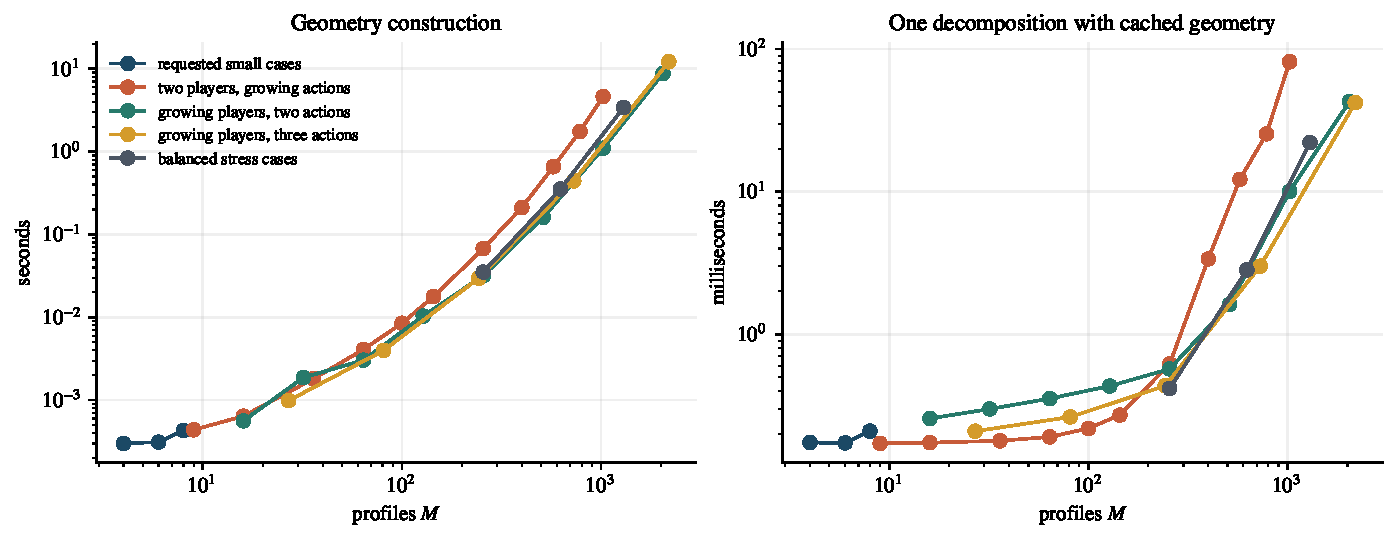
\includegraphics[width=\textwidth]{runtime_by_profiles.pdf}
\caption{Geometry construction and cached decomposition versus the number of
profiles.  Both axes are logarithmic.  Lines connect cases within a controlled
family and are guides to the eye, not fitted complexity models.}
\label{fig:runtime-profiles}
\end{figure}

Figure~\ref{fig:isolated-scaling} isolates the two main growth experiments.
For two players, setup grows from $0.64$~ms at $4\times4$ to $4.62$~s at
$32\times32$.  For binary-action games, adding players from four to eleven
increases $M$ from 16 to 2048 and setup from $0.56$~ms to $8.80$~s.  The
logarithmic vertical scale makes the transition from fixed Python overhead on
tiny cases to dense linear-algebra cost on larger cases visible.

\begin{figure}[htbp]
\centering
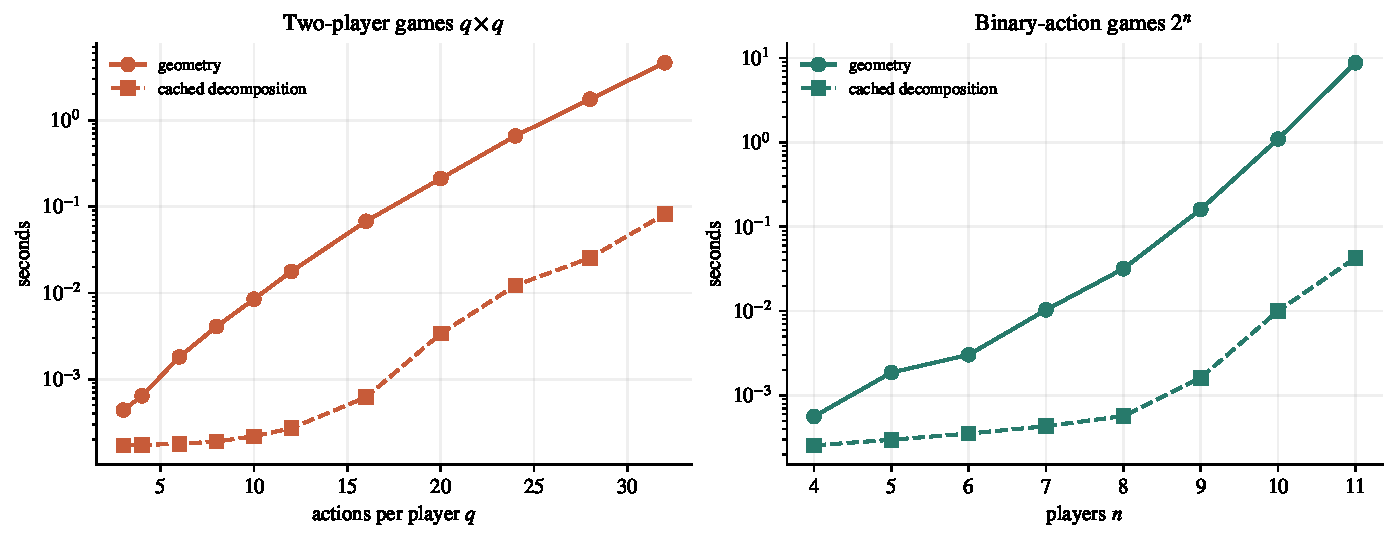
\includegraphics[width=\textwidth]{isolated_scaling.pdf}
\caption{Controlled scaling with actions per player (left) and number of
players (right).  The vertical axes are logarithmic.}
\label{fig:isolated-scaling}
\end{figure}

Persistent numerical storage follows the dimension formula closely, as shown
in Figure~\ref{fig:storage}.  The largest executed case, $3^7$, stores about
548~MiB of NumPy arrays and requires 12.15~s for its single measured geometry
construction.  The $3^8$ successor would require approximately 5.45~GiB for
the leading persistent arrays alone and was therefore not allocated.  This is
the practical stopping point of the present dense experiment.

\begin{figure}[htbp]
\centering
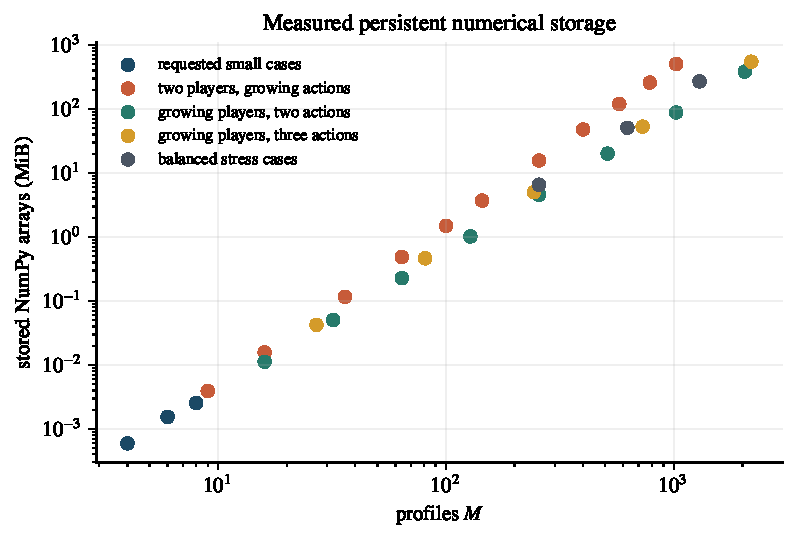
\includegraphics[width=0.72\textwidth]{storage_by_profiles.pdf}
\caption{Persistent NumPy storage owned by each constructed geometry.  Both
axes are logarithmic; temporary arrays and Python object overhead are not
included.}
\label{fig:storage}
\end{figure}

\subsection{Numerical validation and interpretation}

For every timed game, the script recomputes a result and records three
residuals.  Across the 30 successful cases, the maximum reconstruction
residual
\[
 \|u-u^{\mathrm N}-u^{\mathrm P}-u^{\mathrm H}\|_\infty
\]
was exactly zero in floating-point arithmetic because the final component is
formed by subtraction.  The largest co-closedness residual
\[
 \|G^*Du^{\mathrm H}\|_\infty
\]
was $1.06\times10^{-12}$, and the largest absolute potential--harmonic game
inner product was $7.67\times10^{-12}$.  These values are consistent with
double-precision eigensolver and matrix-multiplication error at the tested
dimensions.

The data support three computational conclusions.
\begin{enumerate}
 \item Geometry construction is the dominant cost because it forms a dense
       Gram matrix and its pseudoinverse.  Caching changes the relevant bound
       from~\eqref{eq:setup-time} to~\eqref{eq:cached-time}.
 \item Profile count alone is insufficient to predict runtime: edge count
       explains substantial differences between skeletons with the same $M$.
 \item Persistent memory, rather than the time for one cached decomposition,
       becomes the first hard barrier in the present dense design.  A sparse
       operator and a solve-based treatment of the Laplacian are the natural
       route to larger games.
\end{enumerate}
The experiment is descriptive rather than a proof of asymptotic exponents;
the rigorous exponents are those derived from the executed matrix dimensions
in Section~\ref{sec:complexity}.

\subsection{Reproduction}

From the repository root, the committed data and figures can be regenerated
with
\begin{verbatim}
cd CandoganDecomposition/Documentation/experiments
python benchmark_decomposition.py
python plot_benchmarks.py
\end{verbatim}
The first command overwrites \path{benchmark_results.csv} and
\path{benchmark_metadata.json}; the second overwrites the PDF/PNG figures and
\path{benchmark_table.tex}.  Timing changes across runs are expected, but the
case definitions, random inputs, matrix dimensions, and numerical residual
checks are deterministic.

\section*{Implementation version}

The implementation analyzed here is the maintained NumPy core as present in
the repository in July 2026.  Its source is
\path{CandoganDecomposition/decomposition.py}.  The benchmark data were
collected on July 15, 2026.  The document and experiment directory are intended
to evolve together if the core is later changed to sparse storage or a
solve-based projection.

\begin{thebibliography}{9}

\bibitem{candogan2011}
O.~Candogan, I.~Menache, A.~Ozdaglar, and P.~A.~Parrilo,
\newblock Flows and decompositions of games: harmonic and potential games,
\newblock \emph{Mathematics of Operations Research} 36 (2011), 474--503.
\newblock \url{https://doi.org/10.1287/moor.1110.0500}.

\bibitem{abdou2022}
J.~Abdou, N.~Pnevmatikos, M.~Scarsini, and X.~Venel,
\newblock Decomposition of games: some strategic considerations,
\newblock \emph{Mathematics of Operations Research} 47 (2022), 1766--1784.

\end{thebibliography}

\end{document}
